\documentclass[cic,tc]{iiufrgs}

% Use unicode
\usepackage[utf8]{inputenc}   % pacote para acentuação

% Necessário para incluir figuras
\usepackage{graphicx}         % pacote para importar figuras

\usepackage{times}            % pacote para usar fonte Adobe Times
% \usepackage{palatino}
% \usepackage{mathptmx}       % p/ usar fonte Adobe Times nas fórmulas

\usepackage[alf,abnt-emphasize=bf]{abntex2cite}	% pacote para usar citações abnt

% 
% Informações gerais
% 
\title{Planejando Viagens: Desenvolvimento do sistema web para planejamento de viagens}

\author{de Souza La Porta}{Henrique}

% orientador e co-orientador são opcionais (não diga isso pra eles :))
\advisor[Prof.~Dr.]{Soares Pimenta}{Marcelo}

% a data deve ser a da defesa; se nao especificada, são gerados
% mes e ano correntes
% \date{maio}{2001}

% o local de realização do trabalho pode ser especificado (ex. para TCs)
% com o comando \location:
% \location{Itaquaquecetuba}{SP}

% itens individuais da nominata podem ser redefinidos com os comandos
% abaixo:
% \renewcommand{\nominataReit}{Prof\textsuperscript{a}.~Wrana Maria Panizzi}
% \renewcommand{\nominataReitname}{Reitora}
% \renewcommand{\nominataPRE}{Prof.~Jos{\'e} Carlos Ferraz Hennemann}
% \renewcommand{\nominataPREname}{Pr{\'o}-Reitor de Ensino}
% \renewcommand{\nominataPRAPG}{Prof\textsuperscript{a}.~Joc{\'e}lia Grazia}
% \renewcommand{\nominataPRAPGname}{Pr{\'o}-Reitora Adjunta de P{\'o}s-Gradua{\c{c}}{\~a}o}
% \renewcommand{\nominataDir}{Prof.~Philippe Olivier Alexandre Navaux}
% \renewcommand{\nominataDirname}{Diretor do Instituto de Inform{\'a}tica}
% \renewcommand{\nominataCoord}{Prof.~Carlos Alberto Heuser}
% \renewcommand{\nominataCoordname}{Coordenador do PPGC}
% \renewcommand{\nominataBibchefe}{Beatriz Regina Bastos Haro}
% \renewcommand{\nominataBibchefename}{Bibliotec{\'a}ria-chefe do Instituto de Inform{\'a}tica}
% \renewcommand{\nominataChefeINA}{Prof.~Jos{\'e} Valdeni de Lima}
% \renewcommand{\nominataChefeINAname}{Chefe do \deptINA}
% \renewcommand{\nominataChefeINT}{Prof.~Leila Ribeiro}
% \renewcommand{\nominataChefeINTname}{Chefe do \deptINT}

% A seguir são apresentados comandos específicos para alguns
% tipos de documentos.

% Relatório de Pesquisa [rp]:
% \rp{123}             % numero do rp
% \financ{CNPq, CAPES} % orgaos financiadores

% Trabalho Individual [ti]:
% \ti{123}     % numero do TI
% \ti[II]{456} % no caso de ser o segundo TI

% Monografias de Especialização [espec]:
% \espec{Redes e Sistemas Distribuídos}      % nome do curso
% \coord[Profa.~Dra.]{Weber}{Taisy da Silva} % coordenador do curso
% \dept{INA}                                 % departamento relacionado

% 
% palavras-chave
% iniciar todas com letras minúsculas, exceto no caso de abreviaturas
% 
\keyword{formatação eletrônica de documentos}
\keyword{\LaTeX}
\keyword{ABNT}
\keyword{UFRGS}

%\settowidth{\seclen}{1.10~}

% 
% inicio do documento
% 
\begin{document}

% folha de rosto
% às vezes é necessário redefinir algum comando logo antes de produzir
% a folha de rosto:
% \renewcommand{\coordname}{Coordenadora do Curso}
\maketitle

% dedicatoria
% \clearpage
% \begin{flushright}
%     \mbox{}\vfill
%     {\sffamily\itshape
%       ``If I have seen farther than others,\\
%       it is because I stood on the shoulders of giants.''\\}
%     --- \textsc{Sir~Isaac Newton}
% \end{flushright}

% agradecimentos
%\chapter*{Agradecimentos}
%Agradeço ao \LaTeX\ por não ter vírus de macro\ldots



% resumo na língua do documento
\begin{abstract}
    Este documento é um exemplo de como formatar documentos para o
    Instituto de Informática da UFRGS usando as classes \LaTeX\
    disponibilizadas pelo UTUG\@. Ao mesmo tempo, pode servir de consulta
    para comandos mais genéricos. \emph{O texto do resumo não deve
      conter mais do que 500 palavras.}
\end{abstract}

% resumo na outra língua
% como parametros devem ser passados o titulo e as palavras-chave
% na outra língua, separadas por vírgulas
\begin{englishabstract}{Using \LaTeX\ to Prepare Documents at II/UFRGS}{Electronic document preparation. \LaTeX. ABNT. UFRGS}
    This document is an example on how to prepare documents at II/UFRGS
    using the \LaTeX\ classes provided by the UTUG\@. At the same time, it
    may serve as a guide for general-purpose commands. \emph{The text in
      the abstract should not contain more than 500~words.}
\end{englishabstract}

% lista de figuras
\listoffigures

% lista de tabelas
\listoftables

% lista de abreviaturas e siglas
% o parametro deve ser a abreviatura mais longa
\begin{listofabbrv}{SPMD}
    \item[JWT] 

\end{listofabbrv}

% idem para a lista de símbolos
% \begin{listofsymbols}{$\alpha\beta\pi\omega$}
%     \item[$\sum{\frac{a}{b}}$] Somatório do produtório
%     \item[$\alpha\beta\pi\omega$] Fator de inconstância do resultado
% \end{listofsymbols}

% sumario
\tableofcontents

% aqui comeca o texto propriamente dito

% introducao

\chapter{Introdução}


\chapter{O Problema}

Atualmente o planejamento de viagens por conta própria, sem necessidade da intervenção de agências de viagens, tem se tornado cada vez mais popular e acessível devido a grande quantidade de informações disponíveis na internet. Porém, para alguns viajantes surge a dificuldade de organizar esse grande volume de dados e os possíveis custos envolvidos, principalmente quando as viagens são longas, incluem mais de um destino e envolvem mais de uma pessoa. Além disso, outra dificuldade é armazenar as diversas informações que serão necessárias durante a viagem de forma prática e acessível.

Dentro desse contexto existe o blog Planejando Viagens, que tem como objetivo ajudar outros viajantes a planejar viagens, através da disponibilização de informações e dicas sobre diversos lugares do mundo. Atualmente os autores do blog utilizam tabelas de Excel como a principal forma de organização de informações durante o planejamento de suas viagens. Entre os dados utilizados estão informações sobre cidades, datas, hospedagem, transportes, atrações turísticas, previsão de custos, entre outros, que são impressos posteriormente para consulta durante a viagem. O controle de custos ao longo da viagem é feito através de anotações no papel feitas diariamente. Nesse processo informações podem ser perdidas ou esquecidas, além de não existir uma facilidade de acesso remoto das informações a qualquer momento.

\chapter{Estado da Arte}
Google travel

Inspirirock

\chapter{A Proposta}
Desenvolvendo o sistema web

Neste capitulo será proposto um sistema com o objetivo de facilitar a organização de informações referentes a roteiros de viagem, hospedagem, transportes, além da criação da estimativas de gastos. Todas essas informações serão editáveis pelo usuário, existindo a possibilidade de adicionar novos dados ao longo do tempo, como os gastos reais que ocorrem durante a viagem. Portanto, se tornando uma plataforma de planejamento, organização e o controle de todas as informações de uma viagem antes, durante e depois da realização da mesma. 

\section{Requisitos e objetivos}

Afim de esclarecer e identificar os objetivos do software, foi realizado o levantamento dos requisitos junto aos proprietários do blog Planejando Viagens.

Definiu-se, portanto que a aplicação deve:

\begin{itemize}
    \item Permitir a construção e edição de roteiros, através da definição de destinos e locais definidos pelo usuário.
    \item Permitir o inserção e edição de hospedagens no roteiro.
    \item Permitir o inserção e edição de passagens no roteiro, sejam aéreas, terrestres, marítimas e etc.
    \item Permitir o inserção, controle e edição de gastos que ocorrem ou podem vir a ocorrer, na execução de um roteiro.
    \item Possibilitar ao usuário a apresentação do roteiro em um mapa, usando os pontos definidos no roteiro.
    \item Permitir que os roteiros sejam armazenados no sistema.
    \item Ter interface responsiva, ou seja, uma interface prática e adaptável a qualquer dispositivo que a acesse seja smartphone, tablet ou pc.

\end{itemize}

\section{Protótipos de baixa fidelidade}
Com objetivo de obter uma visão geral de como desenvolveria a estrutura do front-end do projeto e suas necessidades, foi realizado protótipos de baixa fidelidade, isto é, são protótipos que apresentam a estrutura visual do que se deseja como conceito de funcionamento, mas não trás detalhes de interface como cores, padrões e etc.

\section{Entidades}
Este projeto trabalha com um grupo pequeno de entidades que se resumem às instâncias mais básicas planejadas para a aplicação. A primeira delas representa um destino, ou seja um local ou um endereço a ser visitado no mapa, e portanto deve possuir atributos
referentes a sua localização, sua identificação, ao estado e prioridade. Um objeto Destino
é composto dos seguintes atributos:
\begin{figure}[htp]
\centering
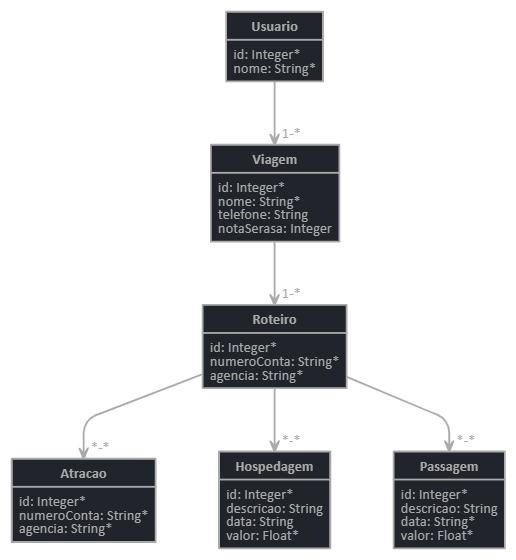
\includegraphics[width=15cm]{tcc/imagens/entidades.png}
\caption{Diagrama de Entidade-Relacionamento}
\label{fig:lion}
\end{figure}

\section{Tecnologias utilizadas}
Para que o projeto fosse desenvolvido foi necessário fazer escolhas de quais tecnologias utilizadas para o desenvolvimento tanto do \textit{back-end} como do \textit{front-end}.

No \textit{back-end} foi utilizado o Strapi um CMS (Content Management Framework) para facilitar o desenvolvimento de API's em \textit{Node.js}, provendo recursos como: Painel de administração, controle de autenticação e permissões, geradores de API, etc. O Strapi é gratuito e \textit{open-source}, podendo ser customizado e estendido livremente. O Strapi agiliza o processo de desenvolvimento, pois provem a criação de tabelas e gerenciamento de autenticação de usuários via JWT.

Para o front-end foi utilizado o framework Nuxt para aplicações em Vue.js.



\chapter{Conclusões}

\chapter{Referências Bibliográficas}

\chapter{Anexos}

% referências
% aqui será usado o environment padrao `thebibliography'; porém, sugere-se
% seriamente o uso de BibTeX e do estilo abnt.bst (veja na página do
% UTUG)
% 
% observe também o estilo meio estranho de alguns labels; isso é
% devido ao uso do pacote `natbib', que permite fazer citações de
% autores, ano, e diversas combinações desses

\bibliographystyle{abntex2-alf}
\bibliography{biblio}

\end{document}
